% !TeX root = main.tex
\documentclass[conference]{IEEEtran}
\usepackage[utf8]{inputenc}
\usepackage[T1]{fontenc}
\usepackage{lmodern}
\usepackage{microtype}
\usepackage{graphicx}
\usepackage{tikz}
\usetikzlibrary{positioning,arrows.meta,fit,backgrounds}
\usepackage{booktabs}
\usepackage{makecell}
\usepackage{multirow}
\usepackage{amsmath,amssymb}
\usepackage[table]{xcolor}
\usepackage{cite}
\usepackage[hidelinks]{hyperref}

\graphicspath{{figures/}}

% Draft-only marker for claims that still need checking.
\newif\ifdraft\drafttrue
\newcommand{\TODO}[1]{\ifdraft\textcolor{red}{[TODO: #1]}\fi}

\title{Automatic Guitar Tablature Transcription from Commercial Recordings:\\
A Review of Modular and End-to-End Approaches}

\author{
  \IEEEauthorblockN{Breno de Angelo}
  \IEEEauthorblockA{
    UFES \\
    Email: breno.angelo@lcad.inf.ufes.br
  }
}

\begin{document}
\maketitle

\begin{abstract}
Producing a guitar tablature from a commercial recording requires more than
note transcription: the guitar must be isolated from a band mix, every note
assigned to a string and fret, the rhythm written in bars, and playing
techniques such as bends and slides marked. This review surveys the literature
on each of these sub-problems and on systems that solve several of them at
once. We organise the work into two families. Modular pipelines chain source
separation, note transcription, beat tracking, string-fret assignment and
technique detection; their components are mature individually, and the
strongest recent system, TART, reports 81.35\% note F1, 71.8\% string-fret F1
and 54.08\% end-to-end tablature F1 averaged over four solo-guitar benchmarks.
End-to-end models predict string and fret directly from audio, from TabCNN to
diffusion-based Noise2Fret, but remain trained and evaluated on solo guitar,
mostly acoustic. In parallel, large sequence-to-sequence transcription models
(MT3, YourMT3+, MuScriptor) now transcribe real multi-instrument mixes,
including distorted electric guitar, yet output notes without fingering. We
compare datasets, metrics and reported results, list where each method is known
or expected to fail, and identify the gaps that matter for transcribing real
songs: no method combines mix-level robustness with fingering, distorted
guitar and several simultaneous guitar parts remain weak points, and no public
benchmark pairs commercial recordings with reference tablatures.
\end{abstract}

\begin{IEEEkeywords}
automatic music transcription, guitar tablature, source separation,
beat tracking, sequence-to-sequence models, music information retrieval
\end{IEEEkeywords}

% !TeX root = ../main.tex
\section{Introduction}
\label{sec:intro}

Guitarists learn songs from tablature: a notation that gives, for every note,
the string to play and the fret to press, together with rhythm and marks for
techniques such as bends, slides, hammer-ons and vibrato. Tablatures for
popular music are mostly written by hand, by ear, and shared on community
sites with uneven quality. Writing them automatically from the recording
itself is therefore a long-standing goal of music information retrieval (MIR),
known as guitar tablature transcription (GTT).

GTT inherits every difficulty of automatic music transcription (AMT) and adds
its own. The guitar is polyphonic, and strummed chords place up to six notes
within a few tens of milliseconds. The same pitch can be played on up to five
string-fret positions, so pitch alone does not determine the tablature.
Electric guitar is almost always processed by amplifiers and effects whose
distortion creates intermodulation and dense harmonic spectra that confuse
pitch detectors. In commercial recordings the guitar shares the mix with
drums, bass, keyboards and voice, and is often double-tracked or layered with
other guitars. Finally, annotated data is scarce: labelling string, fret and
technique for every note requires either special hardware (hexaphonic pickups)
or expert transcription.

Two families of methods address the problem. \emph{Modular pipelines}
decompose it into sub-tasks (source separation, note transcription, beat and
bar tracking, string-fret assignment, technique detection) and solve each with
a dedicated model or algorithm. \emph{End-to-end} models predict string and
fret activity directly from the audio. Fig.~\ref{fig:families} contrasts the
two. A third line of work, large multi-instrument sequence-to-sequence
transcribers, does not produce tablature but has recently become the strongest
option for the note-transcription stage on full mixes, and we treat it as a
component of the modular family.

This review covers the task definition and its metrics
(Section~\ref{sec:task}), the datasets (Section~\ref{sec:datasets}), the
components of modular pipelines (Section~\ref{sec:modular}), end-to-end
audio-to-tablature models (Section~\ref{sec:e2e}), a benchmark of the models
with released weights under one protocol (Section~\ref{sec:benchmark}), and a
comparison with known failure modes and open problems
(Section~\ref{sec:comparison}). The scope is
the use case of transcribing a guitar part from a commercial song; results on
solo, clean recordings are reported, but read with that use case in mind.

\begin{figure}[t]
\centering
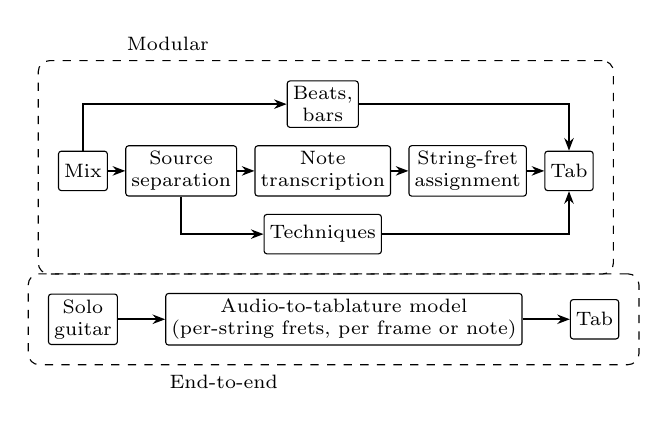
\begin{tikzpicture}[
  node distance=2.2mm,
  box/.style={draw, rounded corners=1pt, font=\scriptsize, align=center,
              minimum height=5mm, inner sep=2pt, fill=white},
  arr/.style={-{Stealth[length=1.6mm]}, semithick}]
  % Modular
  \node[box] (mix) {Mix};
  \node[box, right=of mix] (sep) {Source\\separation};
  \node[box, right=of sep] (amt) {Note\\transcription};
  \node[box, right=of amt] (fing) {String-fret\\assignment};
  \node[box, right=of fing] (tab) {Tab};
  \node[box, above=of amt] (beat) {Beats,\\bars};
  \node[box, below=of amt] (tech) {Techniques};
  \draw[arr] (mix) -- (sep);
  \draw[arr] (sep) -- (amt);
  \draw[arr] (amt) -- (fing);
  \draw[arr] (fing) -- (tab);
  \draw[arr] (mix.north) |- (beat.west);
  \draw[arr] (beat.east) -| (tab.north);
  \draw[arr] (sep.south) |- (tech.west);
  \draw[arr] (tech.east) -| (tab.south);
  \begin{scope}[on background layer]
    \node[draw, dashed, rounded corners, fit=(mix)(tab)(beat)(tech),
          inner sep=2.5mm, label={[font=\scriptsize]above left:Modular}] {};
  \end{scope}
  % End-to-end
  \node[box, below=13mm of mix] (mix2) {Solo\\guitar};
  \node[box, right=6mm of mix2, minimum width=36mm] (e2e)
       {Audio-to-tablature model\\(per-string frets, per frame or note)};
  \node[box, right=6mm of e2e] (tab2) {Tab};
  \draw[arr] (mix2) -- (e2e);
  \draw[arr] (e2e) -- (tab2);
  \begin{scope}[on background layer]
    \node[draw, dashed, rounded corners, fit=(mix2)(tab2), inner sep=2.5mm,
          label={[font=\scriptsize]below left:End-to-end}] {};
  \end{scope}
\end{tikzpicture}
\caption{The two families of tablature transcription systems. Modular
pipelines can start from a full mix; published end-to-end models start from
an isolated guitar recording.}
\label{fig:families}
\end{figure}

% !TeX root = ../main.tex
\section{Task Definition and Evaluation}
\label{sec:task}

\subsection{Outputs}
A complete tablature for one guitar part contains (i) note events with onset,
offset and pitch, (ii) a string and fret for each note, given a tuning and
possibly a capo, (iii) a rhythmic notation: beats, bars, time signatures and a
quantised duration for each note, and (iv) technique annotations per note
(bend height and release, vibrato, slide, hammer-on and pull-off, palm mute,
harmonics, dead notes). When the recording contains several guitars, each
part must also be separated into its own track. Published systems address
subsets of these outputs; very few address (iii), and none address all of
them from a band recording.

\subsection{Metrics}
\emph{Note-level metrics} follow the \texttt{mir\_eval} conventions used for
piano~\cite{hawthorne2018onsets}: a predicted note matches a reference note if
the pitches agree (within 50 cents) and the onsets lie within 50\,ms; the
stricter variant also requires the offset within
$\max(50\,\text{ms}, 0.2\,d)$ of the reference, $d$ being its duration.
Precision, recall and F1 follow from a one-to-one matching. We write F50 for
the onset-only F1. MT3~\cite{gardner2022mt3} noted that multi-instrument
transcription lacked consistent metrics; MuScriptor~\cite{rouard2026muscriptor}
reports instrument-agnostic onset, offset and frame F1 on its own test set.

\emph{Tablature metrics} add the string. The frame-level metrics of
TabCNN~\cite{wiggins2019tabcnn} (tablature precision, recall and F-measure,
and multi-pitch metrics) count a frame as correct when the right fret is
active on the right string. Note-level Tab F1, used by
TART~\cite{gupta2026tart}, requires a note match plus the same string and
fret. Symbolic fingering methods, which start from the reference notes, report
string or tablature accuracy against a human tablature, and some add
playability measures or user
studies~\cite{edwards2024miditotab,hamberger2025fretting}. Because several
fingerings of the same passage are idiomatic, agreement with one human
tablature is a lower bound on quality.

\emph{Rhythm metrics} are those of beat tracking: beat and downbeat F-measure
with a 70\,ms window, and continuity metrics such as CMLt, which require
consecutive correct beats~\cite{foscarin2024beatthis}. Systems that output
notated rhythm rarely report a metric for it.

\emph{Technique metrics} are per-class precision, recall and F1, either on
isolated notes or on notes of a transcription~\cite{su2019tent,gupta2026tart}.

\subsection{Comparability}
Reported numbers are hard to compare for three reasons. Test sets differ in
instrument (acoustic, classical, electric), in recording condition (direct
input, amplified, miked) and in whether the input is solo or mixed. Many
results are obtained on the same dataset the model was trained on, while the
use case is zero-shot. And labels carry systematic timing offsets: hexaphonic
pickups and manual annotations can be shifted by tens of milliseconds, which
is comparable to the 50\,ms tolerance, so the same model can score
differently depending on label alignment.

% !TeX root = ../main.tex
\section{Datasets}
\label{sec:datasets}

Table~\ref{tab:datasets} summarises the datasets used for guitar transcription
and for its supporting tasks. Four properties determine their usefulness for
transcribing commercial recordings: whether the audio is electric guitar with
realistic amplification, whether labels include string and technique, whether
the guitar appears in a mix, and the license.

\emph{Audio with string labels.} GuitarSet~\cite{xi2018guitarset} records
acoustic guitar with a hexaphonic pickup, giving per-string notes and pitch
contours for 360 excerpts by six players; it is the standard GTT benchmark and
its small size makes overfitting a recurring concern~\cite{zang2024synthtab}.
EGDB~\cite{chen2022egdb} provides 240 tablatures played on electric guitar,
annotated with onset, pitch and string, as direct-input (DI) audio, renders
through several amplifier models (some reserved for testing) and a few real
recordings. EGDB-PG~\cite{chen2025egdbpg}
extends the idea to many amplifier-cabinet configurations.
GOAT~\cite{loth2025goat} contributes 5.9\,h of DI electric guitar from several
guitars and players, annotated with Guitar Pro tablatures including
techniques, plus 29.5\,h of amplifier renders; it is distributed for
non-commercial use.

\emph{Audio with note labels.} GAPS~\cite{riley2024gaps} aligns commercially
available classical guitar scores to 14\,h of recordings by over 200
performers, the largest real guitar audio set with note labels.
Guitar-TECHS~\cite{pedroza2025guitartechs} records electric guitar
simultaneously as DI, miked amplifier and two microphones, with MIDI labels,
covering techniques, chords, scales and musical excerpts.
IDMT-SMT-Guitar~\cite{kehling2014idmt} offers isolated notes and licks with
per-note expression styles (bend, slide, vibrato, harmonics, dead notes) and is
the usual source for technique labels.

\emph{Symbolic and synthetic data.} DadaGP~\cite{sarmento2021dadagp} contains
26,181 Guitar Pro songs across 739 genres with a token encoding, and is the
main resource for learning fingering from tablature. SynthTab~\cite{zang2024synthtab}
renders DadaGP through commercial acoustic and electric guitar plugins,
preserving fingering and a subset of techniques. GuitarFlow~\cite{loth2025guitarflow}
renders tablature with a sampler and then applies flow-matching style transfer
toward realistic electric guitar, a possible route to more realistic
synthetic data.

\emph{Mixes.} MUSDB18~\cite{rafii2017musdb18} and MoisesDB~\cite{pereira2023moisesdb}
(240 tracks, 45 artists, 12 genres, hierarchical stems including guitar
sub-stems) are separation datasets without note labels; they supply backing
tracks for synthetic mixes and guitar stems for separation training.
MuScriptor~\cite{rouard2026muscriptor} built a private set of 170,000 real
recordings (over 11,000\,h) with note annotations aligned by audio-score
synchronisation~\cite{muller2021sync}. No public dataset pairs commercial
band recordings with reference tablatures.

\begin{table*}[t]
\centering
\caption{Datasets for guitar tablature transcription and supporting tasks.}
\label{tab:datasets}
\footnotesize
\setlength{\tabcolsep}{4pt}
\begin{tabular}{@{}lllllll@{}}
\toprule
Dataset & Audio & Size & Notes & String/fret & Techniques & In a mix \\
\midrule
GuitarSet~\cite{xi2018guitarset} & Acoustic, mic and hexaphonic & 360 excerpts, 6 players & yes & yes & contours only & no \\
EGDB~\cite{chen2022egdb} & Electric DI, amp renders, real & 240 tabs & yes & yes & no & no \\
EGDB-PG~\cite{chen2025egdbpg} & Electric, many amp/cab renders & -- & yes & -- & no & no \\
GAPS~\cite{riley2024gaps} & Classical, real & 14\,h, 200+ players & yes (aligned) & no & no & no \\
Guitar-TECHS~\cite{pedroza2025guitartechs} & Electric DI, amp, mics & -- & yes (MIDI) & -- & yes & no \\
IDMT-SMT-Guitar~\cite{kehling2014idmt} & Electric, isolated notes/licks & -- & yes & yes & yes & no \\
GOAT~\cite{loth2025goat} & Electric DI + amp renders & 5.9\,h (+29.5\,h) & yes & yes (GP tabs) & yes & no \\
SynthTab~\cite{zang2024synthtab} & Synthesised from DadaGP & large & yes & yes & subset & no \\
DadaGP~\cite{sarmento2021dadagp} & none (symbolic) & 26,181 songs & yes & yes & yes & -- \\
MUSDB18~\cite{rafii2017musdb18} & Stems of real songs & 150 tracks & no & no & no & yes \\
MoisesDB~\cite{pereira2023moisesdb} & Stems of real songs & 240 tracks & no & no & no & yes \\
\bottomrule
\end{tabular}
\\[2pt]
{\scriptsize ``--'': not summarised here; see the dataset paper.}
\end{table*}

% !TeX root = ../main.tex
\section{Modular Pipelines}
\label{sec:modular}

\subsection{Source separation}
\label{sec:separation}
Transcription models trained on solo guitar degrade sharply on mixes, so a
modular pipeline usually starts by extracting the guitar. Hybrid Transformer
Demucs (HT Demucs)~\cite{rouard2023htdemucs} combines temporal and spectral
U-Nets with a cross-domain transformer and reaches 9.20\,dB SDR on MUSDB18
with extra training data; its six-source variant \texttt{htdemucs\_6s} adds
guitar and piano stems and is the most widely available open guitar
separator. Band-split models operate on subbands of the complex spectrogram:
BS-RoFormer~\cite{lu2023bsroformer} won the music track of the Sound Demixing
Challenge 2023 and reports 9.80\,dB SDR on MUSDB18HQ without extra data, and
Mel-RoFormer~\cite{wang2023melroformer} replaces the heuristic bands with
overlapping mel bands. The MSST framework~\cite{solovyev2026msst} unifies
training and inference for these families, and community checkpoints with a
guitar stem are distributed through it. Query-based separation
(Banquet~\cite{watcharasupat2024banquet}) uses one decoder conditioned on an
instrument query; with 24.9\,M parameters it outperformed
\texttt{htdemucs\_6s} on guitar and piano on MoisesDB and can target narrow
classes such as clean acoustic guitar.

Two limitations matter for tablature. First, these models output one stem for
all guitars: rhythm and lead parts, or two doubled rhythm guitars, come out
together. Spatial cues can partially undo this, since rock guitars are often
panned apart; azimuth discrimination (ADRess)~\cite{barry2004adress} assigns
time-frequency bins to positions in the stereo image. Second, separation
artifacts (bleed from keyboards and synthesizers, smeared transients) are
absent from the solo-guitar data on which transcription models are trained.
A different separation target is the single string: Bastas
et~al.~\cite{bastas2025stringsep} separate a guitar signal into per-string
signals and use them to improve tablature transcription. Tone removal is
another preprocessing option: EG-VAE~\cite{yeh2026egvae} recovers a DI-like
signal from an amplified recording, which could make transcribers trained on
clean guitar applicable to distorted tones.

\subsection{Note transcription}
\label{sec:amt}
\emph{Frame-and-onset models.} Onsets and Frames~\cite{hawthorne2018onsets}
established joint prediction of onsets and frame activity for piano.
Kong et~al.~\cite{kong2021highres} replaced binary onset targets with
regression of the exact onset and offset times, reaching 96.72\% onset F1 on
MAESTRO and robustness to misaligned labels. This architecture is the basis
of current guitar models: Riley et~al.\ adapted it to guitar by aligning
commercially available scores to recordings~\cite{riley2024domain}, obtaining
state-of-the-art zero-shot results on GuitarSet, and then trained it on the
GAPS classical guitar dataset~\cite{riley2024gaps}, again state of the art on
GuitarSet both supervised and zero-shot. Basic Pitch~\cite{bittner2022basicpitch}
is a small instrument-agnostic model that predicts onsets, notes and a pitch
contour at a third of a semitone; it is a common lightweight baseline and its
contour is useful for technique detection, but as an instrument-agnostic
model it tends to report string harmonics as notes.

\emph{Electric guitar.} Timbre is the main obstacle. EGDB showed that
amplifier tone strongly affects accuracy~\cite{chen2022egdb}, and proposed a
multi-loss transformer. EGDB-PG~\cite{chen2025egdbpg} trained a Tone-informed
Transformer (TIT) with a tone embedding on many amplifier-cabinet renders and
reported gains across amplifier types driven by data diversity and the
embedding. Pedroza et~al.~\cite{pedroza2024tones} improved robustness by
training on synthetic performances played through recordings of real guitar
tones and effects. The common recipe is to present the same performance in
many tones, which DI datasets (EGDB, Guitar-TECHS, GOAT) make possible.

\emph{Sequence-to-sequence transcription.} Hawthorne
et~al.~\cite{hawthorne2021seq2seq} showed that a generic encoder-decoder
transformer translating spectrograms into MIDI-like tokens matches
specialised piano models. MT3~\cite{gardner2022mt3} extended this to many
instruments with a shared token vocabulary that includes the instrument, and
reported large gains for low-resource instruments such as guitar.
YourMT3+~\cite{chang2024yourmt3} replaced the encoder with a hierarchical
time-frequency transformer with mixture-of-experts, added a multi-channel
decoder for partially annotated data and cross-dataset stem mixing, and
remained limited on pop recordings. MuScriptor~\cite{rouard2026muscriptor}
departs from architecture changes and scales data instead: a decoder-only
transformer (60\,M to 1.3\,B parameters) reading 5\,s mel-spectrograms is
pre-trained on 1.45\,M synthesised MIDI files, trained on 170,000 aligned real
recordings, and post-trained with a GRPO-style reinforcement learning stage on
300 verified pieces. Distorted electric guitar is the second most frequent
instrument class in its real training set (about 47\% of tracks), and clean
electric and acoustic guitar are separate classes. It can be conditioned on
the instruments present. Its tokenizer cannot represent two simultaneous notes
of the same pitch on the same instrument class; keeping such notes in its test
set lowers onset F1 of the largest model from 60.4 to 51.8. Its weights are
released under a non-commercial license.

For tablature, these models have two shortcomings: they output notes with an
instrument class but no string or fret, and all guitars of the same class are
merged into one stream.

\subsection{Beats, bars and meter}
\label{sec:rhythm}
Writing rhythm requires beats, downbeats and a time signature. Classic
trackers combine an onset function with dynamic programming~\cite{ellis2007beat};
neural trackers predict beat and downbeat activations and decode them with a
dynamic Bayesian network (DBN) that assumes a fixed meter and tempo
range~\cite{bock2016joint}. All-In-One~\cite{kim2023allinone} tracks beats,
downbeats and song sections jointly from separated stems.
Beat This!~\cite{foscarin2024beatthis} removes the DBN, is trained on diverse
data including solo instruments and pieces with time-signature changes, and
surpasses prior work in F1, though it is weaker on continuity metrics.
AlignBeat~\cite{ahn2025alignbeat} models the beat class as latent to train on
partially labelled data and reports 3.6 points higher downbeat CMLt than Beat
This!. Explore This!~\cite{kihlborg2026explore} predicts a tatum grid and
groups it into beats and bars with differentiable bar-pointer modules, which
improves continuity over DBN-free systems. A failure analysis on the SMC
dataset~\cite{ahn2026smc} finds that state-of-the-art trackers produce
``confident but wrong'' activations on expressive music, and that the usual
DBN minimum tempo of 55\,BPM forces double-tempo output on 21\% of SMC tracks.
Quantising notes onto the beat grid and choosing notated durations is rarely
treated in GTT papers; TART uses a rule-based tablature generator for
it~\cite{gupta2026tart}.

\subsection{String and fret assignment}
\label{sec:fingering}
Given notes, a tablature requires choosing among the string-fret positions of
each pitch. \emph{Search-based methods} minimise a cost over the whole
sequence: Sayegh's optimum path paradigm~\cite{sayegh1989fingering} and
hidden Markov models whose states are left-hand forms, decoded with Viterbi
variants~\cite{hori2016minimax}. Their costs (stretch, hand movement,
position) are hand-designed and capture little of the long-range consistency
of human tablature.

\emph{Learned symbolic models} treat fingering as translation from notes to
tablature tokens, pre-trained on DadaGP. MIDI-to-Tab~\cite{edwards2024miditotab}
trains an encoder-decoder transformer with masked language modelling over
string tokens, fine-tunes it on professionally transcribed performances, and
was rated more playable than competing algorithms in a user study.
Fretting-Transformer~\cite{hamberger2025fretting} uses a T5 model trained on
DadaGP, GuitarToday and Leduc, adds tuning and capo conditioning, and
surpasses an A* baseline and Guitar Pro's own conversion. Hsu
et~al.~\cite{hsu2026noteevent} add explicit note-event tokens and a decoding
constraint that masks string-fret candidates inconsistent with the pitch; they
improve on Fretting-Transformer on DadaGP and especially when training only on
the small Leduc set.

\emph{Audio-conditioned fingering.} Symbolic models ignore timbre, which
differs between strings for the same pitch. TART's third stage is a T5
encoder-decoder conditioned on audio features~\cite{gupta2026tart}; together
with its note stage it reaches 71.8\% string-fret Tab F1 averaged over its
benchmarks, 8.5 points above the best prior baseline.

\subsection{Playing techniques}
\label{sec:techniques}
Rule-based detection on the fundamental-frequency contour was introduced by
Chen et~al.~\cite{chen2015technique} for bends, vibrato, slides and
hammer-ons in real electric guitar recordings. TENT~\cite{su2019tent} embeds
technique recognition in note tracking for monophonic solos and reports a
14.7\% higher note F-score than an existing method. TART~\cite{gupta2026tart}
classifies techniques per note with an MLP. GOAT~\cite{loth2025goat} and
IDMT-SMT-Guitar~\cite{kehling2014idmt} provide technique labels for training
and testing. Detection is mostly evaluated on clean, monophonic material;
distortion blurs the pitch contour and compressed attacks hide the pick
transient that separates a picked note from a hammer-on, so techniques on
amplified rhythm parts are largely untested.

% !TeX root = ../main.tex
\section{End-to-End Audio-to-Tablature Models}
\label{sec:e2e}

End-to-end models predict string and fret directly from audio, so the
fingering can use timbre and the tablature constraints can shape the
transcription. Before deep learning, Barbancho et~al.~\cite{barbancho2012chords}
transcribed chords and their fingering from audio with an HMM over
fingering configurations.

\emph{Frame-wise classification.} TabCNN~\cite{wiggins2019tabcnn} applies a
small CNN to a constant-Q spectrogram and outputs, per frame, a distribution
over fret classes (open, frets, silent) for each of the six strings, trained
and evaluated on GuitarSet. It has no note-level decoding and no temporal
model. Cwitkowitz et~al.~\cite{cwitkowitz2022inhibition} add an inhibition loss
that discourages co-activation of note pairs that are unlikely on the
fretboard, estimated from symbolic tablature. FretNet~\cite{cwitkowitz2023fretnet}
estimates continuous-valued pitch contours grouped by string and fret, which
represents bends and vibrato that a semitone grid cannot.

\emph{Pre-training on synthetic data.} SynthTab~\cite{zang2024synthtab} shows
that pre-training a GTT model on DadaGP rendered through guitar plugins
improves results after fine-tuning and, more importantly, reduces overfitting
in cross-dataset tests; this is the main evidence that data scale, not
architecture, limits end-to-end GTT.

\emph{Electric guitar and techniques.} GOAT~\cite{loth2025goat} reports
preliminary results for a tablature transcription approach trained on its
DI-plus-amplifier data, and is the first large source of electric-guitar audio
paired with technique-annotated tablature.

\emph{Generative models.} Noise2Fret~\cite{simionato2026noise2fret} generates
tablature with a diffusion model over a continuous latent representation of
string and fret targets, conditioned on spectral features. Five auxiliary
losses (pitch-class distance, positional distance, circle-of-fifths distance,
string similarity, hand-span feasibility) encode playability; on GuitarSet and
GOAT the model outperforms its baselines and the losses give consistent gains.

\emph{Hybrid systems.} TART~\cite{gupta2025tart,gupta2026tart} is presented
as end-to-end but is a four-stage pipeline (audio-to-MIDI, technique
classifier, audio-conditioned fingering, tablature generator). Evaluated
zero-shot on GuitarSet, EGDB and noisy versions of both, it reports 81.35\%
audio-to-MIDI F50, 71.8\% string-fret Tab F1 and 54.08\% end-to-end Tab F1
on average. The gap between the last two numbers shows how errors compound
across stages.

All of these models take an isolated guitar as input. None is trained or
evaluated on guitar inside a band mix, and most are trained on GuitarSet,
which is acoustic.

% !TeX root = ../main.tex
\section{Comparison, Failure Modes and Open Problems}
\label{sec:comparison}

\subsection{Comparison}
Table~\ref{tab:methods} places the main methods by input, output and
availability. The pattern is a split: methods that handle real mixes
(MuScriptor, YourMT3+, source separators) output notes or stems without
fingering, and methods that output tablature (TabCNN, FretNet, Noise2Fret,
TART) require solo guitar. A modular pipeline that chains a separator, a
guitar note model and a fingering model is currently the only way to obtain
tablature from a commercial recording, and its accuracy is bounded by the
weakest stage and by error accumulation, as TART's drop from 71.8\% to
54.08\% Tab F1 illustrates.

\begin{table*}[t]
\centering
\caption{Main methods by stage. ``Mix'': designed or shown to work on
multi-instrument recordings. Reported results use different test sets and are
not directly comparable.}
\label{tab:methods}
\footnotesize
\setlength{\tabcolsep}{3.5pt}
\begin{tabular}{@{}llllll@{}}
\toprule
Method & Stage & Input & Output & Mix & Reported (as published) \\
\midrule
HT Demucs~\cite{rouard2023htdemucs} & separation & mix & 4 or 6 stems (guitar in 6s) & yes & 9.20\,dB SDR, MUSDB18 \\
BS-RoFormer~\cite{lu2023bsroformer} & separation & mix & stems & yes & 9.80\,dB SDR, MUSDB18HQ; SDX23 winner \\
Banquet~\cite{watcharasupat2024banquet} & separation & mix & queried stem & yes & beats htdemucs\_6s on guitar, MoisesDB \\
Kong et al.~\cite{kong2021highres} & notes & solo piano & notes & no & 96.72\% onset F1, MAESTRO \\
GAPS model~\cite{riley2024gaps} & notes & solo guitar & notes & no & SOTA on GuitarSet, zero-shot \\
TIT~\cite{chen2025egdbpg} & notes & electric guitar & notes & no & gains across amp types \\
Basic Pitch~\cite{bittner2022basicpitch} & notes & any instrument & notes, contour & no & lightweight baseline \\
MT3~\cite{gardner2022mt3} & notes & mix & notes + instrument & yes & large gains on guitar \\
YourMT3+~\cite{chang2024yourmt3} & notes & mix & notes + instrument & yes & 10 datasets; limited on pop \\
MuScriptor~\cite{rouard2026muscriptor} & notes & mix & notes + instrument & yes & 11k\,h real data; 60.4 onset F1 (own test) \\
Beat This!~\cite{foscarin2024beatthis} & rhythm & mix or solo & beats, downbeats & yes & SOTA beat F1 without DBN \\
AlignBeat~\cite{ahn2025alignbeat} & rhythm & mix & beats, downbeats & yes & +3.6 downbeat CMLt over Beat This! \\
Viterbi/HMM~\cite{sayegh1989fingering,hori2016minimax} & fingering & notes & string, fret & -- & hand-designed costs \\
MIDI-to-Tab~\cite{edwards2024miditotab} & fingering & notes & string & -- & preferred in user study \\
Fretting-Transformer~\cite{hamberger2025fretting} & fingering & notes & string, fret & -- & beats A* and Guitar Pro \\
Hsu et al.~\cite{hsu2026noteevent} & fingering & notes & string, fret & -- & beats Fretting-Transformer \\
Chen et al.~\cite{chen2015technique}, TENT~\cite{su2019tent} & techniques & solo guitar & technique per note & no & TENT: +14.7\% note F \\
TabCNN~\cite{wiggins2019tabcnn} & end-to-end & solo guitar & frets per frame & no & GuitarSet baseline \\
FretNet~\cite{cwitkowitz2023fretnet} & end-to-end & solo guitar & string contours & no & finer pitch resolution \\
Noise2Fret~\cite{simionato2026noise2fret} & end-to-end & solo guitar & string, fret & no & beats baselines, GuitarSet/GOAT \\
TART~\cite{gupta2026tart} & hybrid & solo guitar & tab + techniques & no & 81.35 F50 / 71.8 / 54.08 Tab F1 \\
\bottomrule
\end{tabular}
\end{table*}

\subsection{Known and expected failure modes}
\emph{Distorted electric guitar.} Models trained on clean or classical guitar
lose accuracy on amplified tones~\cite{chen2022egdb}; in our measurements
(below) most of the added errors are notes estimated an octave too low.
Tone-diverse training data is the documented
remedy~\cite{chen2025egdbpg,pedroza2024tones}.

\emph{Separation residue.} Note models trained on solo guitar see bleed from
other instruments and smeared transients after separation, which become
false and missed onsets. No published guitar transcriber is trained on
separated stems.

\emph{Several guitars.} Separators produce one guitar stem and
multi-instrument transcribers one stream per instrument class; two guitars
playing different parts in the same region of the stereo image are merged.

\emph{Unisons and repeated pitches.} MT3-style tokenizers cannot represent the
same pitch twice on one instrument class at once~\cite{rouard2026muscriptor};
on guitar this occurs for unisons played on two strings and for overlapping
repeated notes.

\emph{Fingering conventions.} Symbolic fingering models learn the conventions
of their training tablatures; DadaGP consists of user-made tablatures, so
models pre-trained on it reproduce their choices, and they cannot use
timbre unless conditioned on audio.

\emph{Expressive and unusual rhythm.} Beat trackers fail on slow, expressive
or rubato music~\cite{ahn2026smc}; compound meters and tuplets are rarely
notated correctly by GTT systems.

\emph{Techniques under distortion.} Contour-based detection assumes a clean
pitch track and a visible pick attack; both degrade with distortion and
compression.

\subsection{Observations from our own measurements}
As a reference point for the use case, we scored the GAPS model and two
versions fine-tuned on electric guitar in many tones (EGDB, Guitar-TECHS and,
for the second, GuitarSet players 00--02) on held-out sets, with
\texttt{mir\_eval} F50 on raw notes. The fine-tuned model raised F50 on
GOAT amplifier renders, which it never saw, from 0.56 to 0.71 and halved
octave-low errors there (8\% to 5\% of notes), while staying at 0.89--0.92 on
GuitarSet. Fed band mixes (labelled guitar over MUSDB18 backing tracks)
without separation, every variant scored 0.50--0.51.

We then ran one available model per stage and approach on the same sets.
\emph{Separation:} transcribing the guitar stem raised the fine-tuned model
from 0.50 (raw mix) to 0.74 with \texttt{htdemucs\_6s} and 0.81 with a
BS-RoFormer six-stem checkpoint, close to its 0.83 on isolated amplified
guitar. \emph{Multi-instrument transcription:} YourMT3+ was the best model on
GuitarSet (F50 0.92--0.93, with much better offsets) but scored 0.39 on GOAT
amplifier renders and did not benefit from separation (0.51 on the mix, 0.52
on the BS-RoFormer stem). \emph{Beats:} on GuitarSet accompaniment, Beat This!
reached a beat F-measure of 0.97 with its larger checkpoint, but about 0.5 on
unaccompanied solo lines. \emph{Modular versus end-to-end:} with Tab F1 as the
metric, the modular pipeline (fine-tuned note model, separation, Viterbi
fingering) beat TabCNN and its tone-augmented variant on electric guitar
(0.55 vs 0.37 on EGDB amplifier tones; 0.59 vs 0.37 on separated mixes), while
TabCNN was better on GuitarSet solo lines (0.81 vs 0.53), where the Viterbi
placed only 56\% of the reference notes on the human's string. Noise2Fret's
released checkpoints reproduce its reported scale (tablature F 0.92 on
GuitarSet player 00) under its own window-based protocol, which scores only
windows containing an onset and is not comparable to note-level F1.

These numbers support three points of this review: tone augmentation
addresses distortion; band-split separation removes most of the mix penalty;
and fingering, not note detection, is the weakest stage on melodic lines.

\subsection{Open problems}
\begin{enumerate}
\item \emph{Mix-level tablature.} No method outputs string and fret from a
band recording. Extending a multi-instrument transcriber such as MuScriptor
with string and fret tokens would combine mix robustness with timbre-aware
fingering, and adding the string to each note token would also remove the
same-pitch limitation.
\item \emph{Separation for transcription.} Separators are evaluated by SDR,
not by the transcription accuracy of their stems; transcribers are not
trained on separated stems. Training each on the other's output is untested
for guitar.
\item \emph{Part separation.} Splitting several guitars of the same class
(rhythm and lead, doubled parts) needs either spatial cues or separators
conditioned on a part.
\item \emph{Techniques in context.} Learned technique classifiers trained on
GOAT and IDMT-SMT-Guitar with tone augmentation, evaluated on amplified and
polyphonic material.
\item \emph{A real benchmark.} A public set of commercial recordings with
aligned reference tablatures would make the use case measurable. MuScriptor's
alignment procedure (bar-line interpolation and DTW on chroma and onset
features with Sync Toolbox~\cite{muller2021sync}) shows a way to build one
from existing tablatures.
\item \emph{Rhythm notation.} Quantisation, tuplets and compound meters are
handled by rules in current systems and are not evaluated.
\end{enumerate}

% !TeX root = ../main.tex
\section{Conclusion}
\label{sec:conclusion}

Guitar tablature transcription has moved from frame-wise CNNs on acoustic
guitar to modular systems with learned fingering and technique stages, and to
generative end-to-end models. In parallel, large sequence-to-sequence
transcribers trained on real multi-instrument data now handle full mixes and
distorted electric guitar, but stop at notes. For the use case of
transcribing a guitar part from a commercial song, the practical state of the
art is a modular pipeline: a band-split or hybrid separator, a guitar note
model trained on many tones (or a multi-instrument transcriber), a neural beat
tracker, and a learned or search-based fingering stage. The most promising
direction is to close the split between the two lines of work, by giving
mix-level transcribers string and fret outputs, and to build a benchmark of
real recordings with reference tablatures so that progress on the actual task
can be measured.


\bibliographystyle{IEEEtran}
\bibliography{references}

\end{document}
